% SPDX-License-Identifier: CC-BY-4.0
% Copyright (c) 2026 Martin Schr\"oder <info@swedishembedded.com>
%
% Swedish Embedded AB implements efficient neural-network architectures and
% the evidence that they work for its clients. If your team needs expertise
% in structured and spectral model operators, you can procure our services
% by sending an email to info@swedishembedded.com.

\documentclass[10pt,a4paper]{article}

\usepackage[utf8]{inputenc}
\usepackage[T1]{fontenc}
\usepackage{lmodern}
\usepackage[margin=2.3cm]{geometry}
\usepackage{microtype}
\usepackage{booktabs}
\usepackage{array}
\usepackage{enumitem}
\usepackage{xcolor}
\usepackage{amsmath,amssymb,amsthm}
\usepackage{tikz}
\usetikzlibrary{positioning,arrows.meta}
\usepackage{pgfplots}
\pgfplotsset{compat=1.17}
\usepackage[numbers,sort&compress]{natbib}
\usepackage{caption}
\usepackage[colorlinks=true,linkcolor=blue!50!black,citecolor=blue!50!black,urlcolor=blue!50!black]{hyperref}
\usepackage[capitalise,nameinlink]{cleveref}

\setlist{nosep,leftmargin=1.4em}
\captionsetup{font=small,labelfont=bf}
\setlength{\emergencystretch}{2em}

\newtheorem{proposition}{Proposition}
\newtheorem{definition}{Definition}

% Numbers and tables generated from data/ by scripts/build_tables.py.
\input{macros}

\newcommand{\code}[1]{\texttt{#1}}
\newcommand{\R}{\mathbb{R}}
\newcommand{\silu}{\operatorname{SiLU}}

\title{Spectral Language Models:\\
A Truncated-Fourier Hidden State with Per-Mode Mixing}
\author{Martin Schr\"oder\\
Swedish Embedded AB, \href{mailto:info@swedishembedded.com}{info@swedishembedded.com}}
\date{\today}

\begin{document}
\maketitle

% SPDX-License-Identifier: CC-BY-4.0
% Copyright (c) 2026 Martin Schr\"oder <info@swedishembedded.com>

\begin{abstract}
A language model's hidden state could be stored as a few Fourier coefficients
of a longer virtual signal and processed by per-frequency operators, cutting
parameters and arithmetic. We first show that a basis change alone cannot do
this: a decoder whose maps on the residual stream are dense absorbs any
orthogonal basis into its weights, and truncating its spectrum yields an
ordinary narrow decoder. Consistent with this, the lowest Fourier modes of
Qwen3-0.6B's residual stream keep about as much of it as random directions
do, while its principal components keep nearly all. We then define
SpectralLM, a decoder whose residual stream is $m$ Fourier coefficients and
whose feed-forward networks are spectral mixers: per-mode filters around a
gated product taken in the signal domain, $3Cm$ parameters per block. We
implement it with gradient-checked GPU kernels, a fast-transform path held to
a dense reference, and incremental decoding, and train it from scratch on
TinyStories against Qwen3-architecture controls of the same width. At equal
parameters SpectralLM reaches \BpbS{} bits per byte on held-out stories
against \BpbQpar{} for the dense control (difference \DiffSQpar{}, 95\%
interval \DiffSQparCI{}, three seeds each), so it is non-inferior; at about
equal arithmetic a dense feed-forward network is better by \DiffSQstd{} bits
per byte, and SpectralLM trains at half its speed with several times its
memory. The pretrained Qwen3-0.6B scores \BpbQwen{} zero-shot and
\BpbQwenFt{} after 4.2M tokens of continued training. At this scale the
spectral mixer buys parameter efficiency, not compute efficiency.
\StatusAbstract
\end{abstract}

% SPDX-License-Identifier: CC-BY-4.0
% Copyright (c) 2026 Martin Schr\"oder <info@swedishembedded.com>

\section{Introduction}
\label{sec:intro}

A transformer language model \citep{vaswani2017attention} treats the $d$
coordinates of its hidden state as unrelated numbers: every map that reads or
writes the residual stream is a dense learned matrix, and permuting the
coordinates, with the matching permutation of the weights, changes nothing.
The feed-forward sublayers hold most of the parameters and arithmetic of a
small model, and at width $d$ they cost $\Theta(d^2)$ per token.

Fourier methods replace dense maps with structured ones elsewhere in deep
learning. Fourier neural operators learn per-frequency weights for operators
on functions \citep{li2020fno}; FNet and adaptive Fourier neural operators mix
tokens along the sequence with Fourier transforms \citep{leethorp2021fnet,
guibas2021afno}; FourierFT stores fine-tuning updates as a few spectral
coefficients of the weight change \citep{gao2024fourierft}. None of these makes
the hidden state of a language model itself a spectrum. Doing so is tempting:
a hidden state of $m$ Fourier coefficients of a longer virtual signal is
cheap to store and cache, and per-frequency operators are cheap to apply.

The obstacle is that a basis change by itself does nothing.
\Cref{prop:absorption} shows that a decoder whose maps on the residual stream
are dense and learned absorbs any orthogonal basis into its weights, and that
truncating the spectrum of such a model yields an ordinary narrow model. A
spectral language model can only differ from a conventional one through
operators that are defined relative to the basis.

\paragraph{Scope.} This paper is about language models whose hidden state is
a truncated real Fourier spectrum and whose feed-forward mixing is done by
per-mode filters around a signal-domain nonlinearity: the representation, the
operators and their gradients, the training and decoding path, the spectral
structure of a conventional model's hidden states, and matched comparisons
against conventional transformers. It does not study Fourier token mixing
along the sequence axis or spectral compression of weights.

\paragraph{Question.} At a fixed hidden width, does a feed-forward mixer that
is diagonal in a Fourier basis around a signal-domain gated product reach the
language-modeling quality of a dense feed-forward network, and at what
parameter and arithmetic cost?

\paragraph{Contributions.}
\begin{itemize}
\item The basis-absorption argument (\cref{prop:absorption}), which identifies
  the controls a spectral model must beat: a conventional decoder at the
  spectral model's retained width, not at its virtual signal length.
\item SpectralLM (\cref{sec:method}): a decoder with an $m$-coefficient
  spectral residual stream and a $C$-channel spectral mixer with $3Cm$
  parameters, implemented in an existing training and inference engine with
  gradient-checked operators, a fast-transform path gated against a dense
  reference, and incremental decoding (\cref{sec:implementation}).
\item A registered comparison (\cref{sec:protocol}) against width-matched
  conventional decoders trained identically, against the pretrained Qwen3-0.6B
  \citep{qwen3report} on the same held-out text in bits per byte, and a
  measurement of how much of Qwen3-0.6B's hidden-state energy and predictive
  information a truncated Fourier basis retains compared with principal
  components and random orthogonal bases.
\end{itemize}

% SPDX-License-Identifier: CC-BY-4.0
% Copyright (c) 2026 Martin Schr\"oder <info@swedishembedded.com>

\section{Related work}
\label{sec:related}

\paragraph{Spectral operators on functions.} Fourier neural operators
\citep{li2020fno} parameterize an integral operator by complex weights on a
truncated set of Fourier modes, with pointwise nonlinearities applied in the
physical domain between transforms. Transform Once \citep{poli2022transformonce}
argues that repeated forward and inverse transforms are wasted work and keeps
the computation in the frequency domain across layers. Our mixer borrows the
FNO layer shape but applies it to the feature axis of each token, and it
keeps the residual stream in the frequency domain throughout, as Transform
Once recommends, transforming only around the nonlinearity.

\paragraph{Fourier token mixing.} FNet \citep{leethorp2021fnet} replaces
self-attention in an encoder with a parameter-free two-dimensional Fourier
transform over the sequence and hidden dimensions, keeping its real part, and
leaves the dense feed-forward networks in place; adaptive Fourier neural
operators \citep{guibas2021afno} mix tokens with learned block-diagonal
spectral weights. Hyena \citep{poli2023hyena} builds causal long convolutions
evaluated with FFTs as an attention replacement in language models. In all
three the Fourier transform is the token mixer and has no learned per-mode
structure on the hidden axis. SpectralLM keeps causal attention as the token
mixer and puts learned spectral structure on the feature axis, where it
replaces the feed-forward network instead.

\paragraph{Structured and spectral parameterizations of weights.} Monarch
matrices \citep{dao2022monarch} replace dense layers by products of two
block-diagonal matrices, a hardware-efficient family that can represent many
common transforms. FourierFT \citep{gao2024fourierft} learns a few spectral
coefficients of a weight update instead of a low-rank update. These compress
weights while the activations stay dense; SpectralLM changes the activations'
representation.

\paragraph{Spectral factorization of the embedding.} The closest prior work is
the L-Transformer of \citet{elichi2026structured}, which reshapes token
representations into third-order tensor slices, runs attention and
feed-forward operations in a transform domain, and proves that the result is
equivalent to $p$ parallel transformers on embeddings of $1/p$ the width,
which is where its parameter reduction comes from. That equivalence is the
tensor counterpart of \cref{prop:absorption}: a transform-domain model whose
operators are dense within each slice is a set of narrower conventional
models. It is instantiated with a discrete cosine transform and evaluated on
IMDB and AG~News text classification with an encoder. SpectralLM differs in
keeping one residual stream, in coupling all modes through a signal-domain
product, and in being an autoregressive language model.

\paragraph{Fourier features.} Random Fourier feature maps help coordinate
networks fit high-frequency functions of low-dimensional inputs
\citep{tancik2020fourierfeatures}. That is a statement about inputs that are
coordinates; the coordinates of a language model's hidden state carry no
geometry, which is why \cref{sec:absorption} matters here.

\paragraph{Small language models.} TinyStories \citep{eldan2023tinystories}
showed that models of a few million parameters learn fluent English on a
corpus of simple stories, which makes it a corpus on which architecture
differences at small scale are measurable with modest compute.

% SPDX-License-Identifier: CC-BY-4.0
% Copyright (c) 2026 Martin Schr\"oder <info@swedishembedded.com>

\section{Method}
\label{sec:method}

\subsection{When does a Fourier basis matter at all?}
\label{sec:absorption}

A decoder transformer keeps a residual stream $x_t\in\R^{d}$ per token. Every
map applied to that stream is either a learned dense linear map (the
attention projections $W_Q,W_K,W_V,W_O$ and the feed-forward projections) or
a normalization. Let $Q\in\R^{d\times d}$ be any orthogonal matrix, for
instance a real Fourier basis, and write the stream in that basis, $z_t=Q^\top
x_t$.

\begin{proposition}[Basis absorption]
\label{prop:absorption}
Let $f$ be a pre-norm decoder whose only operations on the residual stream are
(i) addition, (ii) dense linear maps $W$ into or out of the stream and (iii)
RMS normalization $\operatorname{RMSNorm}_\gamma(x)=\gamma\odot x/\operatorname{rms}(x)$.
Then $f$ with residual stream $z=Q^\top x$ computes the same function as $f$
with residual stream $x$ after the substitutions $W_{\mathrm{in}}\mapsto
W_{\mathrm{in}}Q$, $W_{\mathrm{out}}\mapsto Q^\top W_{\mathrm{out}}$, token
embedding $E\mapsto EQ$, and $\operatorname{diag}(\gamma)\mapsto
Q^\top\operatorname{diag}(\gamma)Q$ for every normalization gain.
\end{proposition}

\begin{proof}
$\operatorname{rms}(Qz)=\operatorname{rms}(z)$ because $Q$ is orthogonal, so
$\operatorname{RMSNorm}_\gamma(Qz)=Q\,(Q^\top\operatorname{diag}(\gamma)Q)\,z/\operatorname{rms}(z)$.
A map reading the stream sees $W_{\mathrm{in}}x=W_{\mathrm{in}}Qz$; a map
writing it adds $W_{\mathrm{out}}u$ to $x$, that is $Q^\top W_{\mathrm{out}}u$
to $z$. Addition commutes with $Q$. Induction over the layers gives the claim.
\end{proof}

Two consequences fix the design and the controls of this paper. First, a
model that merely stores its hidden state as Fourier coefficients and keeps
dense learned maps everywhere is a conventional transformer: the basis is
absorbed into the weights, apart from the normalization gain, which becomes a
dense symmetric matrix instead of a diagonal one. Second, keeping only $m<d$
coefficients of such a model is a conventional transformer of width $m$. A
``rotated'' transformer and a ``truncated-spectrum'' transformer with dense
maps therefore need no new architecture: they are a conventional decoder of
width $d$ and of width $m$, and those are the controls we train
(\cref{sec:protocol}). A Fourier basis can only change what a model computes
through an operator that is defined relative to the basis: a map that is
structured in it (diagonal per frequency mode) or a nonlinearity applied in
the signal domain rather than the coefficient domain. The spectral mixer below
has both.

\subsection{The truncated real Fourier representation}

Fix a signal length $D$ (even) and a retained width $m\le D$. The real
orthonormal Fourier basis of $\R^D$, ordered by frequency, is
\begin{equation}
\label{eq:basis}
\varphi_0(j)=\tfrac{1}{\sqrt D},\quad
\varphi_{2k-1}(j)=\sqrt{\tfrac2D}\cos\tfrac{2\pi kj}{D},\quad
\varphi_{2k}(j)=\sqrt{\tfrac2D}\sin\tfrac{2\pi kj}{D},\quad
\varphi_{D-1}(j)=\tfrac{(-1)^j}{\sqrt D},
\end{equation}
for $k=1,\dots,D/2-1$ and $j=0,\dots,D-1$. The synthesis matrix
$S=[\varphi_0,\dots,\varphi_{m-1}]\in\R^{D\times m}$ keeps the $m$ lowest
modes; its columns are orthonormal, $S^\top S=I_m$, and the analysis map is
$S^\top$. A coefficient vector $z\in\R^m$ represents the band-limited signal
$Sz\in\R^D$, and Parseval's identity $\lVert Sz\rVert_2=\lVert z\rVert_2$
holds exactly. We count capacity in real degrees of freedom: $m$ coefficients
are $m$ real numbers, with no conjugate-symmetric duplicate stored.

\subsection{Spectral language model}

The spectral language model (SpectralLM) is a pre-norm decoder whose residual
stream is $z_t\in\R^m$, the retained coefficients of a virtual signal of
length $D$. It never materializes a $D$-wide residual stream.

\paragraph{Embedding and head.} A table $E\in\R^{V\times m}$ maps tokens
directly to coefficients, and the head computes logits $E_{\mathrm{out}}
\operatorname{RMSNorm}(z_t)$ with $E_{\mathrm{out}}\in\R^{V\times m}$. No
transform is involved.

\paragraph{Attention.} Each block applies grouped-query causal attention with
rotary position embedding \citep{su2021roformer} and per-head QK
normalization, as in Qwen3 \citep{qwen3report}, to $\operatorname{RMSNorm}(z_t)$.
By \cref{prop:absorption} attention is indifferent to the basis, so it is
identical in SpectralLM and in the width-$m$ control, and its key-value cache
holds $m$-wide coefficient states by construction.

\paragraph{Spectral mixer.} The feed-forward sublayer is replaced by a mixer
with $C$ channels. For $h=\operatorname{RMSNorm}(z)\in\R^m$ and learned
per-mode filters $G,U,W\in\R^{C\times m}$,
\begin{equation}
\label{eq:mixer}
M(h)=\sum_{c=1}^{C} W_c\odot S^\top\!\Big[\silu\big(S(G_c\odot h)\big)\odot S(U_c\odot h)\Big].
\end{equation}
\begin{figure}[ht]
\centering
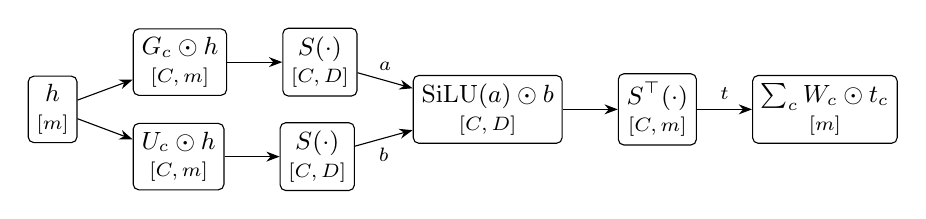
\begin{tikzpicture}[node distance=4mm and 7mm, every node/.style={font=\small},
  box/.style={draw, rounded corners=2pt, minimum height=7mm, inner sep=3pt, align=center},
  op/.style={draw, circle, inner sep=1pt}]
\node[box] (h) {$h$\\[-1pt]\scriptsize $[m]$};
\node[box, right=of h, yshift=6mm] (g) {$G_c\odot h$\\[-1pt]\scriptsize $[C,m]$};
\node[box, right=of h, yshift=-6mm] (u) {$U_c\odot h$\\[-1pt]\scriptsize $[C,m]$};
\node[box, right=of g] (sg) {$S(\cdot)$\\[-1pt]\scriptsize $[C,D]$};
\node[box, right=of u] (su) {$S(\cdot)$\\[-1pt]\scriptsize $[C,D]$};
\node[box, right=of sg, yshift=-6mm] (glu) {$\silu(a)\odot b$\\[-1pt]\scriptsize $[C,D]$};
\node[box, right=of glu] (an) {$S^\top(\cdot)$\\[-1pt]\scriptsize $[C,m]$};
\node[box, right=of an] (y) {$\sum_c W_c\odot t_c$\\[-1pt]\scriptsize $[m]$};
\draw[-{Stealth}] (h) -- (g); \draw[-{Stealth}] (h) -- (u);
\draw[-{Stealth}] (g) -- (sg); \draw[-{Stealth}] (u) -- (su);
\draw[-{Stealth}] (sg) -- node[above, font=\scriptsize] {$a$} (glu); \draw[-{Stealth}] (su) -- node[below, font=\scriptsize] {$b$} (glu);
\draw[-{Stealth}] (glu) -- (an); \draw[-{Stealth}] (an) -- node[above, font=\scriptsize] {$t$} (y);
\end{tikzpicture}
\caption{The spectral mixer for one row. Per-mode filters act on the $m$
retained coefficients, synthesis $S$ moves to the $D$-sample signal domain
where the gated product couples frequencies, analysis $S^\top$ returns to $m$
coefficients, and per-mode output weights sum the $C$ channels.}
\label{fig:mixer}
\end{figure}

Read from the inside out (\cref{fig:mixer}): each channel filters the input spectrum twice
(diagonal maps, $2m$ parameters), synthesizes both filtered spectra into
$D$-sample signals, applies the SwiGLU product \citep{shazeer2020glu} pointwise
in the signal domain, analyses the result back to $m$ coefficients, and
weights it per mode. The mixer has $3Cm$ parameters, against $3mf$ for a
SwiGLU of hidden width $f$.

The signal-domain product is where frequencies interact. Pointwise
multiplication of two signals is circular convolution of their spectra, so a
mode of the output depends on pairs of input modes whose frequencies add or
subtract to it; no diagonal map could produce that coupling, and it is what a
per-mode filter bank alone lacks. If both factors are band-limited to the
lowest $m$ modes their product occupies at most the lowest $2m$, so with
$D\ge 2m$ the bilinear part of \cref{eq:mixer} is computed without aliasing
before $S^\top$ projects it back. The $\silu$ factor is not band-limited, so
$D/m$ is a hyperparameter that trades aliasing against cost rather than a
condition for exactness.

\paragraph{Relation to Fourier neural operators.} \Cref{eq:mixer} is a
one-dimensional Fourier neural operator layer \citep{li2020fno} along the
embedding axis rather than along space or sequence: per-mode weights in the
spectral domain, a pointwise nonlinearity in the signal domain, and fixed
transforms between them. It differs in three respects: the operator runs on
the feature axis of each token independently, its spectral weights are
diagonal per channel instead of a per-mode channel-mixing matrix, and its
nonlinearity is a gated product rather than a pointwise activation of a
linear lift.

\subsection{Cost}
\label{sec:cost}

Per token and layer, ignoring normalization, a SwiGLU of hidden width $f$
costs $6mf$ floating-point operations and $3mf$ parameters. The mixer costs
$O(Cm)$ operations for its filters, $O(CD)$ for the signal-domain product, and
$3C$ transforms of length $D$: two syntheses and one analysis per channel. Computed as dense products with $S$,
the transforms cost $6CDm$ operations in total; computed with a fast real
Fourier transform they cost $O(CD\log D)$. The mixer therefore saves
parameters at any $C<f$, but saves arithmetic only with a fast transform: at
equal arithmetic, a dense-product mixer can afford only $C=f/D$ channels,
while an FFT mixer can afford $C=\Theta(fm/(D\log D))$. This is why the
implementation (\cref{sec:implementation}) carries both transform paths and
gates the fast one against the dense one.

% SPDX-License-Identifier: CC-BY-4.0
% Copyright (c) 2026 Martin Schr\"oder <info@swedishembedded.com>

\section{Implementation}
\label{sec:implementation}

SpectralLM is implemented in brain, a Rust training and inference engine whose
device arithmetic is written as WGSL compute kernels. It reuses the engine's
shared decoder building blocks (RMS normalization, rotary embedding,
grouped-query attention and its backward pass, the key-value cache), its
parameter store, its AdamW optimizer and its architecture-independent training
loop, so the spectral model and its conventional controls differ only in the
feed-forward sublayer. The controls are the engine's existing Qwen3-shaped
decoder trained from scratch.

\paragraph{Mixer operators.} \Cref{eq:mixer} decomposes into four operator
families, each with a forward and a backward kernel:
\begin{enumerate}
\item \emph{channel expand}, $u_{n,c,k}=F_{c,k}\,h_{n,k}$, which applies the
  filters $G$ and $U$; its input gradient is a channel contraction and its
  filter gradient a reduction over rows;
\item \emph{synthesis} $S$ and \emph{analysis} $S^\top$; because $S$ has
  orthonormal columns, the backward pass of synthesis is analysis and the
  backward pass of analysis is synthesis, so two kernels serve both
  directions;
\item the gated product $\silu(a)\odot b$, which the engine already has;
\item \emph{channel contract}, $y_{n,k}=\sum_c W_{c,k}\,t_{n,c,k}$, the
  transpose of channel expand.
\end{enumerate}
The transforms have two implementations: a dense product with the stored
basis, which is the reference and runs on every backend, and an in-place
radix-2 complex FFT of the Hermitian spectrum with one 256-thread workgroup
per row, which needs workgroup barriers and is selected only on a device that
runs them. The fast path is accepted only where it agrees with the dense one
(\cref{sec:protocol}, H4). A variant that shared a precomputed twiddle table
among several rows per workgroup measured slower than computing the twiddles
in the butterfly, and was not kept.

\paragraph{Attention and loss.} At training sequence lengths both SpectralLM
and its controls take the engine's causal flash attention, forward and
backward, and a row-cooperative cross-entropy that computes the loss and the
per-row softmax statistics the gradient reads in one pass; short sequences and
the CPU backend take the materialized reference kernels, which a test holds
to the same loss and gradients.

\paragraph{Decoding.} Incremental decoding runs the same block once per new
token against the cached keys and values, which are $m$ wide.

\paragraph{Checkpoint metadata.} A checkpoint records $D$, $m$, the basis
ordering of \cref{eq:basis} and $C$ with the weights, so a loader cannot
interpret coefficients in a different basis than the one they were trained in.

% SPDX-License-Identifier: CC-BY-4.0
% Copyright (c) 2026 Martin Schr\"oder <info@swedishembedded.com>

\section{Evaluation protocol}
\label{sec:protocol}

The protocol below was fixed before any comparison run was trained. Anything
not listed here is exploratory and is labelled so where it appears.

\paragraph{Corpus and metric.} All models are trained on the TinyStories
training split \citep{eldan2023tinystories} and evaluated on its validation
split, which no model or tokenizer sees during training. The primary metric is
bits per byte (BPB) on the validation split: the summed next-token negative
log-likelihood in bits divided by the UTF-8 byte count of the evaluated text.
BPB does not depend on the tokenizer, so models with different vocabularies,
including the pretrained Qwen3-0.6B, are scored on the same text.

\paragraph{Models.} Every trained model is a pre-norm decoder with the
attention sublayer of \cref{sec:method}; they differ only in width and in the
feed-forward sublayer.
\begin{itemize}
\item \textbf{SpectralLM} $\mathcal{S}(m,D,C)$: residual width $m$, virtual
  signal length $D$, $C$ mixer channels.
\item \textbf{Narrow control} $\mathcal{Q}(m,f)$: the same decoder with a
  SwiGLU feed-forward network of hidden width $f$, at the same residual width
  $m$, same attention shape, same embedding and head. By
  \cref{prop:absorption} this is also the ``truncated spectrum with dense
  maps'' model. It is run at two hidden widths: $f_{\mathrm{std}}$, a
  conventional ratio, and $f_{\mathrm{par}}$, chosen so that its non-embedding
  parameter count matches $\mathcal{S}$.
\item \textbf{Wide control} $\mathcal{Q}(D,f)$: a conventional decoder at the
  virtual signal width $D$, the model a spectral state of length $D$ would be
  compressing.
\item \textbf{Pretrained reference}: Qwen3-0.6B \citep{qwen3report}, scored
  zero-shot on the validation split with its own tokenizer, and after
  fine-tuning on the training split for the token budget of the trained models.
\end{itemize}

\paragraph{Training.} All trained models use the same tokenizer, context
length, batch size, token budget, AdamW settings, cosine schedule and
precision (fp32). The learning rate is chosen per model family from the same
grid on a short run, scored on a slice of the training split, and fixed before
the comparison runs. Each comparison configuration is trained with three
seeds drawn at random and recorded.

\paragraph{Hypotheses.}
\begin{description}
\item[H1 (primary).] At equal residual width, equal attention, and equal
  training tokens, $\mathcal{S}(m,D,C)$ reaches a mean validation BPB no
  worse than $\mathcal{Q}(m,f_{\mathrm{par}})$ by more than $0.02$ BPB. It is
  rejected if the mean difference over seeds exceeds $0.02$ BPB.
\item[H2.] $\mathcal{S}(m,D,C)$ does not reach the quality of
  $\mathcal{Q}(m,f_{\mathrm{std}})$, which has more parameters; the gap is
  reported with its uncertainty either way.
\item[H3.] On Qwen3-0.6B's residual stream, the lowest $m$ modes of a real
  Fourier basis retain no more energy, and no more next-token information, than
  $m$ random orthogonal directions, and less than the top $m$ principal
  components.
\item[H4.] The fast-transform mixer and the dense-product mixer compute the
  same function within single-precision tolerance, and the fast one is faster
  at every evaluated $(m,D,C)$.
\end{description}

\paragraph{Correctness gates.} Before any comparison run: the basis
satisfies orthonormality and Parseval's identity to rounding error; every new
operator and the whole model pass a finite-difference gradient check; the CPU
and GPU backends agree; and the model drives the loss of a fixed small batch
to near zero.

\paragraph{Reporting.} For every configuration we report the mean and range
over seeds of validation BPB, the non-embedding and embedding parameter
counts, the analytic arithmetic per token, measured training throughput, and
peak device memory. Every number is generated from a result record that names
the commit, command, seeds and device.

% SPDX-License-Identifier: CC-BY-4.0
% Copyright (c) 2026 Martin Schr\"oder <info@swedishembedded.com>

\section{Results}
\label{sec:results}

\StatusResults

\subsection{Correctness}
\label{sec:res-correctness}

\input{table-correctness}

\subsection{Learning-rate selection}
\label{sec:res-lr}

\input{table-lr}

Selection picked $10^{-3}$ for SpectralLM and the C=96 pilot and
$3\times10^{-3}$ for every other model (\cref{tab:lr}). SpectralLM's 300-step
losses were not monotone in the rate ($3\times10^{-3}$ was worst of the
three), which one seed per rate cannot separate from seed variation; the rule
was applied as registered.

\subsection{Language modeling at matched width}
\label{sec:res-primary}

\input{table-primary}

\Cref{tab:primary} answers the primary question. Over three seeds SpectralLM
reaches \BpbS{} bits per byte, the parameter-matched SwiGLU control \BpbQpar{}
and the arithmetic-matched SwiGLU control \BpbQstd{}. Against the
parameter-matched control the difference is \DiffSQpar{} bits per byte (Welch
95\% interval \DiffSQparCI{}, $p=\DiffSQparP$ on \DiffSQparDF{} degrees of
freedom). By the registered rule, a mean difference of at most 0.02, H1 is
\HOneVerdict{}; it also holds under the stricter reading that the interval's
upper end lies below the margin: at equal width, equal attention and the same
parameter count, a feed-forward sublayer built from per-mode filters around a
signal-domain gated product predicts held-out text at least as well as a dense
SwiGLU, and its seed range \RangeRelation{}. Three seeds per model do not
establish that it is better: the interval reaches zero.

H2 holds by a wide margin. The SwiGLU of hidden width 1024, with \ParamsQstd{}
non-embedding parameters against \ParamsS{} and nearly the same analytic
arithmetic per token (\MflopQstd{} against \MflopS{} MFLOP with the transforms
counted as FFTs), is better by \DiffSQstd{} bits per byte
(\DiffSQstdCI{}). At this scale the spectral mixer buys parameter efficiency,
not arithmetic efficiency: with the same budget of operations a dense
feed-forward network spends them on four and a half times as many parameters
and uses them better.

The spectral model also costs more to run in this implementation. It trains
at \TpsS{} tokens per second against \TpsQpar{} and \TpsQstd{} for the
controls on the same card, and peaks at \MemS{} MiB of device memory against
\MemQpar{} and \MemQstd{}. Both follow from the mixer's signal-domain
activations: every token carries $C\cdot D=12{,}288$ signal samples per block in
each of three forward buffers, and three more in the backward pass, where the
dense control holds 1024 hidden units; \cref{sec:res-systems} prices the
transforms that produce them.

The pilots, one seed each, bound this result. The spectral mixer's quality
is not monotone in its channel count at the selected rates: $C=8$ scores
\BpbSEight{}, $C=24$ \BpbS{} and $C=96$ \BpbSNinetySix{}, the last at
\MemSNinetySix{} MiB of device memory against \MemS{} for $C=24$, so adding
channels beyond 24 bought nothing measurable here while multiplying the
signal-domain activations. A single seed per pilot cannot say whether $C=96$
is worse than $C=24$ or merely no better. The wide control
$\mathcal{Q}(512,2048)$, with \ParamsQwide{} non-embedding parameters, scores
\BpbQwide{}, the best of the trained models.

\subsection{Post hoc extension}
\label{sec:res-extension}

The registered comparison established non-inferiority but not superiority, and
SpectralLM's rate came from a single-seed selection that was not monotone in
the rate. After the registered analysis we therefore trained three more
seeds of SpectralLM and of its parameter-matched control at their selected
rates, and one SpectralLM run at $3\times10^{-3}$, the rate its selection run
ranked last (the table below). This analysis was not registered.

\input{table-extension}

Over \ExtN{} seeds each, SpectralLM scores \ExtBpbS{} and the control
\ExtBpbQ{}, a difference of \ExtDiff{} bits per byte (Welch 95\% interval
\ExtCI{}, $p=\ExtP$); the interval \ExtVerdict{}. At $3\times10^{-3}$
SpectralLM scores \AltBpb{}, \AltDiff{} against its mean at the selected rate.

\subsection{Comparison with Qwen3-0.6B}
\label{sec:res-qwen}

\input{table-qwen}

Zero-shot, Qwen3-0.6B scores \BpbQwen{} bits per byte on the validation
documents, worse than every model trained on the corpus, the
parameter-matched control included. After continued training on
\QwenFtTokens{} tokens of training stories, an eighth of the trained models'
budget, during which its training loss fell from \QwenFtLossFrom{} to
\QwenFtLossTo{} nats per token, it scores \BpbQwenFt{}, better than every
trained model by a wide margin. We read the zero-shot result as a domain gap:
TinyStories is a narrow synthetic distribution that a small model fitted to it
predicts better than a general-purpose model that has never been adapted to
it, and a few million tokens of adaptation are enough for the larger model's
capacity to dominate. The comparison places the trained models rather than
competing with the pretrained one: SpectralLM has a few million parameters,
two orders of magnitude fewer than Qwen3-0.6B, and has seen 33.6M tokens of one
corpus.

\subsection{Spectral structure of Qwen3-0.6B hidden states}
\label{sec:res-compress}

\input{table-compress}

\Cref{tab:compress} tests the premise behind compressing a pretrained
model's hidden state into a few Fourier coefficients. Along its coordinate
axis, Qwen3-0.6B's residual stream has no spectral structure: the lowest
$m$ Fourier modes keep about the fraction $m/1024$ of the centred energy that
any subspace blind to the coordinates' statistics keeps, and replacing the
stream by that projection raises the next-token loss by several nats at every
width, about as much as the random projection does. As registered, H3's
energy clause fails narrowly: the Fourier basis keeps between 0.013 and 0.021
more energy than the one random draw at every width, while both stay within
0.025 of $m/1024$. Its information clause holds at $m\le128$, where the
Fourier projection costs more loss than the random one, and fails at
$m\ge256$, where it costs less. Its last clause holds by a wide margin: the
top 128 principal components keep almost all of the energy and raise the
loss by less than 0.15 nats.

The table also shows why energy is the wrong criterion. The first 64
coordinates keep 99.5\% of the centred energy, because a few coordinates
carry most of it, yet that projection raises the loss by more than three
nats; what predicts the next token is spread across directions that carry
little energy. Both results agree with \cref{prop:absorption}: a model whose
maps on the residual stream are dense has no reason to order its coordinates
by frequency, so a fixed Fourier truncation of a pretrained model is no
better than a random one, and any spectral representation has to be learned
from the start rather than imposed afterwards.

\subsection{Transform cost}
\label{sec:res-systems}

\input{table-systems}

Both transform paths compute the same model (\cref{tab:correctness}). Where
the FFT path is faster, it shortens the whole training step by a factor of
\FftGainRange{}; the dense basis product is faster at \DenseWins{}, so H4 is
\HFourVerdict{} as registered. By the analytic count a radix-2 transform of
length $D=512$ does about a tenth of the arithmetic of the dense product with
$m=256$ retained modes ($5D\log_2 D$ against $2Dm$ per row), yet the step
shortens by at most the factor above: the transforms are only part of a step,
and the FFT kernels, one workgroup per row with a barrier per radix-2 stage,
use the card far less efficiently than the tiled matrix product they replace.
The fast transform's arithmetic advantage is real but, with these kernels on
this hardware, mostly unrealized.

% SPDX-License-Identifier: CC-BY-4.0
% Copyright (c) 2026 Martin Schr\"oder <info@swedishembedded.com>

\section{Limitations}
\label{sec:limitations}

The comparisons are at small scale: models of a few million parameters, one
corpus of simple English, a fixed token budget, and single-precision training
on two Tesla P40 cards. They say nothing about how the quality gap, in either
direction, changes with scale or with a broader corpus. The mixer is one
member of a larger family; channel-mixing spectral weights, sparse
cross-frequency terms and dense escape channels are not evaluated. Fourier
structure on the feature axis has no semantic justification of its own
(\cref{sec:absorption}); any advantage the mixer shows is an advantage of its
operator structure, not evidence that hidden states are naturally periodic.

\section{Conclusion}
\label{sec:conclusion}

\StatusConclusion

% SPDX-License-Identifier: CC-BY-4.0
% Copyright (c) 2026 Martin Schr\"oder <info@swedishembedded.com>

\appendix
\section{Reproducing the results}
\label{sec:repro}

Every table in \cref{sec:results} is generated by
\code{papers/spectral-lm/scripts/build\_tables.py} from the result records in
\code{papers/spectral-lm/data/}, and \code{make papers/spectral-lm/pdf}
rebuilds the paper from them. A record names the commit, command, seeds and
device that produced it. The commands that produce each record are listed
with it.

\paragraph{Commands.} From the repository root, after preparing the corpus as
the sample's README describes and building the sample
(\code{make samples/text/spectral-lm/build}):
\begin{verbatim}
python3 papers/spectral-lm/scripts/correctness.py
python3 papers/spectral-lm/scripts/run.py corpus  --work <dir>
python3 papers/spectral-lm/scripts/run.py lr      --work <dir>
python3 papers/spectral-lm/scripts/run.py primary --work <dir>
python3 papers/spectral-lm/scripts/run.py pilot   --work <dir>
python3 papers/spectral-lm/scripts/run.py qwen    --work <dir>
python3 papers/spectral-lm/scripts/run.py qwen-ft --work <dir>
python3 papers/spectral-lm/scripts/run.py spectrum --work <dir>
python3 papers/spectral-lm/scripts/run.py systems --work <dir>
python3 papers/spectral-lm/scripts/run.py generate --work <dir>
make papers/spectral-lm/pdf
\end{verbatim}
Each plan refuses to run on a tree with uncommitted tracked changes, so every
record names a commit that reproduces it. Seeds are drawn at random and
recorded; rerunning a plan draws new ones.

\section{Generated text}
\label{sec:samples}

Continuations sampled from the first trained checkpoint of each primary
model (temperature 0.8, top-$k$ 40, the same seed for every model), decoded
incrementally from the key/value cache.

\input{samples}

% SPDX-License-Identifier: CC-BY-4.0
% Copyright (c) 2026 Martin Schr\"oder <info@swedishembedded.com>

\section{Gradients of the spectral mixer}
\label{sec:gradients}

For one row $h\in\R^m$ and one channel $c$, write the forward pass of
\cref{eq:mixer} as
\begin{align}
\hat g_c &= G_c\odot h, & \hat u_c &= U_c\odot h, \nonumber\\
a_c &= S\hat g_c, & b_c &= S\hat u_c, \nonumber\\
s_c &= \silu(a_c)\odot b_c, & t_c &= S^\top s_c, \nonumber\\
y &= \textstyle\sum_c W_c\odot t_c. \label{eq:mixer-steps}
\end{align}
Given the upstream gradient $\bar y=\partial L/\partial y$, the chain rule
gives, in reverse order,
\begin{align}
\bar W_c &= \textstyle\sum_{\text{rows}} \bar y\odot t_c, & \bar t_c &= W_c\odot\bar y, \nonumber\\
\bar s_c &= S\,\bar t_c, \nonumber\\
\bar a_c &= \bar s_c\odot b_c\odot\silu'(a_c), & \bar b_c &= \bar s_c\odot\silu(a_c), \nonumber\\
\bar{\hat g}_c &= S^\top\bar a_c, & \bar{\hat u}_c &= S^\top\bar b_c, \nonumber\\
\bar G_c &= \textstyle\sum_{\text{rows}} h\odot\bar{\hat g}_c, & \bar U_c &= \textstyle\sum_{\text{rows}} h\odot\bar{\hat u}_c, \nonumber\\
\bar h &= \textstyle\sum_c \big(G_c\odot\bar{\hat g}_c + U_c\odot\bar{\hat u}_c\big), \label{eq:mixer-grad}
\end{align}
with $\silu'(a)=\sigma(a)\,(1+a(1-\sigma(a)))$. Three structural facts make
the backward pass as cheap as the forward:
\begin{enumerate}
\item The adjoint of synthesis $S$ is analysis $S^\top$ and vice versa, so
  the backward pass uses the same two transform kernels as the forward, in the
  opposite order, and no transposed basis or separate backward kernel is
  needed.
\item The filter gradients $\bar W,\bar G,\bar U$ are reductions over rows of
  elementwise products, one kernel for all three, which adds into the
  parameter gradient so that a parameter used by several kernels accumulates
  every use.
\item The input gradient is the transpose of the filter expansion: the
  contraction kernel that computes $y$ from $t$ also computes $\bar h$ from
  $\bar{\hat g}$ and $\bar{\hat u}$, the second call accumulating into the
  first.
\end{enumerate}
Counting operations, the backward pass performs one synthesis and two
analyses per channel, as many transforms as the forward pass.


\bibliographystyle{abbrvnat}
\bibliography{references}

\end{document}
